\documentclass[11.5pt]{sig-alternate} % sets document style to sig-alternate
% packages
% typesetting
%\usepackage{dirtytalk} % typset quotations easier (\say{stuff})
\usepackage{hanging} % hanging paragraphs
\usepackage[defaultlines=3,all]{nowidow} % avoid widows
\usepackage[pdfpagelabels=false]{hyperref} % produce hypertext links, includes backref and nameref
\usepackage{xurl} % defines url linebreaks, loads url package
\usepackage{microtype}
\usepackage{textgreek}
%\usepackage{textcomp}
%\newcommand{\texttildemid}{\raisebox{0.4ex}{\texttildelow}}
% layout
\usepackage{enumitem} % control layout of itemize, enumerate, description
\usepackage{fancyhdr} % control page headers and footers
\usepackage{float} % improved interface for floating objects
%\usepackage{multicol} % intermix single and multiple column pages
% language
\usepackage[utf8]{inputenc} % accept different input encodings
\usepackage[english]{babel} % multilanguage support
% misc
\usepackage{graphicx} % builds upon graphics package, \includegraphics
%\usepackage{lastpage} % reference number of pages
%\usepackage{comment} % exclude portions of text (?)
\usepackage{xcolor} % color extensions
\usepackage[backend=biber, style=apa]{biblatex} % sophisticated bibliographies % necessary for HTML to display author info and date on abstract page
\usepackage{csquotes} % advanced quotations, makes biblatex happy
\usepackage{authblk} % support for footnote style author/affiliation
% tables and figures
\usepackage{tabularray}
%\usepackage{array} % extend array and tabular environments
\usepackage{caption} % customize captions in figures and tables (rotating captions, sideways captions, etc)
%\usepackage{cuted} % allow mixing of \onecolumn and \twocolumn on same page
\usepackage{multirow} % create tabular cells spanning multiple rows
%\usepackage{subfigure} % deprecated, support for manipulation of small figures
%\usepackage{tabularx} % extension of tabular with column designator "x", creates paragraph-like column whose width automatically expands
%\usepackage{wrapfig} % allows figures or tables to have text wrapped around them
%\usepackage{booktabs} % better rules
% dummy text
%\usepackage{blindtext} % blind text dummy text
%\usepackage{kantlipsum} % Kant style dummy text
\usepackage{lipsum} %lorem ipsum dummy text
% other helpful packages may be booktabs, longtable, longtabu, microtype

\pagestyle{fancy} % sets pagestyle to fancy for fancy headers and footers

% header and footer
% modern way to set header image
\renewcommand{\headrulewidth}{0pt} % defines thickness of line under header
\renewcommand{\footrulewidth}{0pt} % defines thickness of line above header
\setlength\headheight{80.0pt} % sets height between top margin and header image, effectively moves page contents down
\addtolength{\textheight}{-80.0pt} % seems to affect the lower height. maybe only works properly if footer numbers enabled?
\fancyhf{}
\fancyhead[CE, CO]{
\includegraphics[width=\textwidth]{headerImage.png}}
% footer
%\fancyfoot[LE,LO]{Article Title Here \\ DOI: }% left footer article title and doi
%\fancyfoot[CE,CO]{{}} % center footer empty
%\fancyfoot[RE,RO]{\thepage} % right footer page numbers
%\pagenumbering{arabic} % arabic (1, 2, 3) numbering in footer

\hypersetup{colorlinks=true,urlcolor=blue} % sets link color to blue
\urlstyle{same} % sets url typeface to same as rest of text

% set caption and figure to italics, label bold, left align captions, does not transfer to HTML
\captionsetup{labelfont=bf, font={large, it}, justification=raggedright, singlelinecheck=false}
\renewcommand\theContinuedFloat{\alph{ContinuedFloat}}

%this next bit is confusing, but essentially changes the width of the abstract. Seems to have been copied from this https://tex.stackexchange.com/questions/151583/how-to-adjust-the-width-of-abstract
\let\oldabstract\abstract
\let\oldendabstract\endabstract
\makeatletter %changes @ catcode to enable modification (in parsep)
\renewenvironment{abstract} %alters the abstract environment
{\renewenvironment{quotation}%
               {\list{}{\addtolength{\leftmargin}{1em} % change this value to add or remove length to the the default ?
                        \listparindent 1.5em%
                        \itemindent    \listparindent%
                        \rightmargin   \leftmargin%
                        \parsep        \z@ \@plus\p@}%
                \item\relax}%
               {\endlist}%
\oldabstract}
{\oldendabstract}
\makeatother %changes @ catcode to disable modification

% checks
% italics 
% links 
% dashes 
% tildes 
\begin{document}

\title{Teaching Physics to Deaf College Students In A 3-D Virtual Lab}

\author[1]{\large \color{blue}Vicki Robinson}

\affil[1]{Rochester Institute of Technology/ National Technical Institute for the Deaf}

\toappear{}
%% ABSTRACT
\maketitle
\begin{@twocolumnfalse} 
\begin{abstract}
\item 
\textit{Virtual worlds are used in many educational and business applications. At the National Technical Institute for the Deaf at Rochester Institute of Technology (NTID/RIT), deaf college students are introduced to the virtual world of Second Life, which is a 3-D immersive, interactive environment, accessed through computer software. NTID students use this virtual environment to practice concepts first encountered in the laboratory.}
\\ \\
Keywords: science, physics, virtual world, Second Life, 3D environment.
\end{abstract}
\end{@twocolumnfalse}

%% AUTHOR INFORMATION

\textbf{*Corresponding Author,Vicki Robinson }\\
\href{mailto: vicki.robinson@rit.edu }{(vicki.robinson@rit.edu)} \\
\textit{Submitted  Nov 3 2014}\\
\textit{Accepted Nov 14 2014} \\
\textit{Published online Nov 14 2014} \\
\textit{DOI:10.14448/jsesd.06.0003} \\
\pagebreak
\clearpage
\begin{large}
\section*{PROLOGUE}
Nash, a college freshman, turns his attention to his physics homework. It’s well below zero degrees outside. The wind is howling, and snow is blowing. It’s 1:00 AM, and Nash is dressed comfortably, with a cup of coffee at his side, and his laptop in front of him. On the laptop screen his “avatar,” a young man in jeans and a t-shirt, the legend “Nash001” floating above his head, flies between two large white brick buildings, and lands neatly on a mahogany platform laid over a lawn. Nash001 (Fig. 1) represents Nash in a virtual world, existing in a computer server somewhere, and rendered on Nash’s computer screen. Two other avatars are there, a female vampire and a squirrel, and they all chat for a while. The vampire is Nash’s lab partner’s avatar, and a classmate controls the squirrel. These students see what Nash sees on their own computer screens, but from the perspective of their own avatars. Each avatar interacts with this virtual world and the other avatars under the control of the human student at the computer.

\begin{figure}[h]
    \centering
    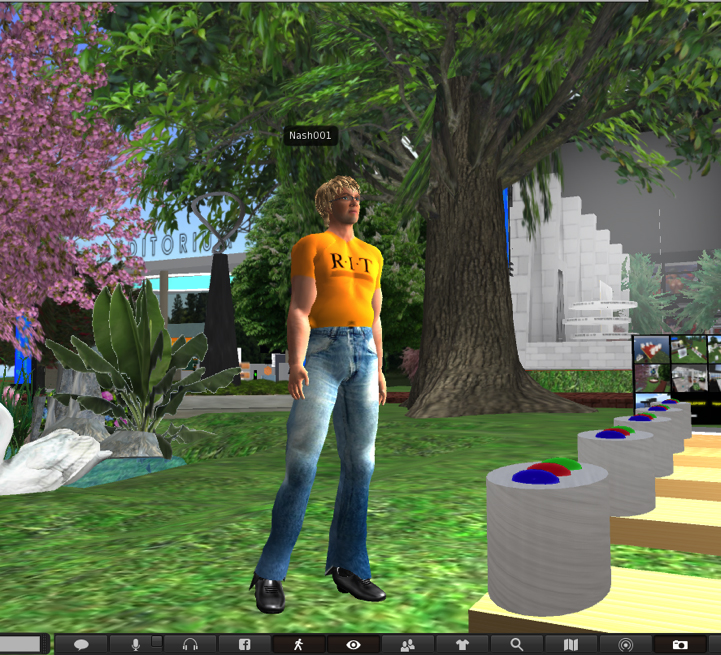
\includegraphics[width=1\linewidth]{fig 1.jpg}
    \caption{Nash001}
\end{figure}
\section*{INTRODUCTION}

Physics teachers want their students to learn physics. Physics students want a good grade in physics. This article will share an application of a new technology that can give everybody what they want.

A virtual world is “a user-defined world where people can interact, play, build 3D objects, do business, and communicate.” (Edwards, 2006) Often thought of in terms of gaming, virtual “grids” offer users the opportunity to build structures, create art and music, and collaborate in any number of activities through “avatars,” personalized personae that can move, communicate, and interact with the virtual environment and other avatars. Second Life is one example of a virtual world, and it is the largest, with well developed graphics and in-world physics that govern the behavior of objects and avatars. Boellstorff (2008) explains “The residents of Second Life create communities, buy property and build homes, go to concerts, meet in bars, attend weddings and religious services, buy and sell virtual goods and services, find friendship, fall in love--the possibilities are endless, and all encountered through a computer screen.” Second Life is owned by a commercial entity, Linden Labs. Avatars are created free of charge, and participation in most Second Life events is also free. Building in Second Life requires a paid “Premium” membership. Students using teacher- or institution-owned property are not charged. In 2009, Rochester Institute of Technology (RIT) created a presence (“RIT Island”) in the virtual world of Second Life in order to allow faculty to explore new learning activities in virtual space. Several teaching faculty at RIT experimented with using Second Life as a teaching or creative space. Second Life can offer advantages to any physics student, primarily the ability to interact with an environment in three dimensions and to do so without any need for highly specialized equipment. Students only need access to a computer with appropriate viewer software that is available without cost from a number of sources, so when RIT instructors were invited to propose projects, a plot of land was requested for physics classes at the National Technical School For The Deaf at RIT (NTID/RIT). The kinds of activities that could be created were discussed with the staff at Online Learning (later Wallace Memorial Library), and thus “Oddprofessor’s Museum and Science Center” was born. This project’s needs quickly outgrew the small plot that was provided on RIT Island, so a modestly larger plot on the Second Life mainland was procured outside of RIT Island. As a result, the original scope of the project rapidly expanded. When RIT discontinued its support for a presence in Second Life in 2011, a large parcel on Second Life’s “mainland” was already equipped with activities both in place and under development. Oddprofessor’s Museum and Science Center on the mainland region of Mujigae comprised more than 23 000 m2 (5.7 acres) of virtual land as of the winter of 2014. (Fig. 2)

\begin{figure}[h]
    \centering
    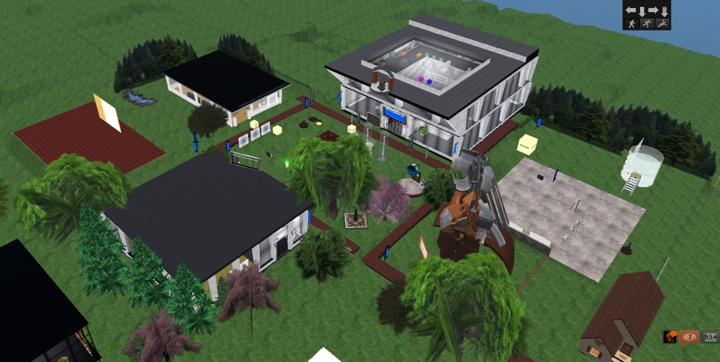
\includegraphics[width=1\linewidth]{fig 2.jpg}
    \caption{An aerial view of the Science Center. The Center comprises about 23,000 square
meters of virtual real estate.}
\end{figure}

\section*{RATIONALE}

To a mature learner it might seem obvious that homework, class work, and hands-on lab experience should ideally form a cohesive whole, with each dimension supporting and expanding the other two. This understanding is at the heart of active learning. “The core elements of active learning are student activity and engagement in the learning process. Active learning is often contrasted to the traditional lecture where students passively receive information from the instructor.” (Prince 2004) Science instructors have long used lab work as active learning, and physics instruction at NTID/RIT was no different. Students attended class, did labs, and did homework, all with the goal that engagement in the learning process would happen, and that each of these elements would serve to enhance the others.

Despite the best of intentions, the learning outcomes did not always realize the ideal. A number of students seemed to compartmentalize knowledge according to which learning activity seemed to be most salient overall, usually homework. When questions referring to lab activities turned up on exams, a small number of students were taken off guard, and sometimes complained that matters were being unfairly complicated. These students were equally baffled when they were directed to their text or the previous day’s demonstrations or discussions to answer their questions in the laboratory. They appeared to have difficulty integrating lab experiences with homework problems. Domin (1999) describes the lecture/lab format used with these students, which followed a very traditional lecture-lab-homework-evaluation plan, as one that does not encourage students’ thinking.

To help break down this compartmentalization, it was necessary to relate homework and test problems to lab work in a way that students could better use. Of course, the connections existed and were evident to the instructor, but often were opaque to the student. Limited, shared lab space and equipment, and time constraints made an increase in lab time not feasible.

Lord and Orkwiszewski (2006 p. 342) describe at length a classroom in which the teacher is in complete charge, the students are disengaged, waiting for instructions without curiosity or participation. This might be a way of doing labs that too many science lab instructors can instantly (and uncomfortably) recognize. Students also recognize this kind of lab but are seemingly comfortable with it. This “sage on the stage” approach may be boring, but it is safe. Ambiguity is the enemy, and in a population wherein communication is one of the primary classroom challenges, students often request specificity. Marschark and Knoors (2012) cite literature that show that both children and university students who are deaf do not demonstrate a spontaneous use of prior knowledge to solve problems. This can pose a significant barrier to active learning as Prince (2004) defines it; there is nothing engaging about it. Students can flounder, often unable to understand what they are to do. They have requested clear, minutely detailed lab protocols to follow, which is consistent with the dependent learning style described by Lang, et. al. (1998). They have remarked that homework is “easier” than lab work. Perhaps this is because homework problems are unambiguous; the parameters of the solution are defined, and the right answer is attainable.

Wieman and Perkins (2005) point out that “peripheral information” (information that is not germane to the problem being investigated, although it is present in the lab environment,) is ignored by the instructor in a class, but may be confusing to students who do not know yet what is a tree, and what is a forest. In a real-life lab, this perplexity is unavoidable, and the instructor watches out for signs of the “teachable moment.” The serendipitous errors that occur in real-life lab activities are valuable parts of the learning process, but those errors are made in the presence of a knowledgeable mentor. Students who are unsure to start with end up confused and frustrated when something unexpected happens when they are on their own. Even worse, they may be unaware that their results are anomalous, and simply carry on in obedience to the lab instructions. One of the jobs of an instructor, particularly in an active learning environment, is to peer over the students’ shoulders and say “Are you sure about that?”

Given that students are not skilled judges of what is important and what is not, the results of any practical lab experience that is performed as homework must be predictable and replicable in an environment that is out of the teacher’s control; the dorm, the library, a student’s home at 3:00 AM. For a virtual lab, controlling the activity is important, and can be “[...] done by enhancing certain features, hiding others, adjusting time scales, and so on, until the desired student perception is achieved.” (Wieman and Perkins, 2005)

In virtual space, instructors have a great deal of control over the students’ experiences. dos Santos (2009) describes the Havok physics “engine” in Second Life as providing “the most realistic virtual environment in the market.” but points out some of the ways in which Second Life physics deviates from reality and therefore needs to be explicitly controlled. Usually, in simple cases illustrating Newtonian mechanics, the physics of the virtual world is close enough to that of the real world for most purposes. Where the virtual physics diverges from the real world in significant and sometimes dismaying ways, there are techniques to make sure that users of an activity get the results that the teacher wants them to get. For example, Second Life has no analog for the physical concept of “liquid.” The behavior of objects submerged in liquid and the “liquid” itself must be carefully scripted in simulations of buoyancy and volume displacement.

Virtual labs can change the dynamic that exists among the students as well as between the students and the instructor. Merchant et. al. (2014) found in a meta-analysis of research on the effectiveness of the educational use of simulations that simulations that offered students the opportunity to practice a concept which they had first encountered in another medium were more effective than simulations used in isolation. Second Life can therefore be seen as an opportunity to create a 3-D lab experience that could be sent home with students after they have completed a physical lab activity in order to bridge the perceptual gap between real-life lab work and homework. Students can do virtual labs anywhere they happen to be as long as they have a properly equipped computer and an Internet connection. Lab work in physics classes at NTID/RIT students are free to use the virtual equipment any way they want to, and to use it as often as they want to. Collaboration is easy; students can meet to work together even if they live miles apart, at any time, and in any weather. The text-based communication function in Second Life means that students with varying communication needs and skills can communicate with each other quite well and it is possible to archive the “chat” in Second Life for review at a later time. Instructors can structure the site to send themselves an e-mail notification when an avatar enters the Second Life plot, so they can “teleport” their avatars to the students’ location to answer questions or pose queries. This work can be done late at night and on weekends if desired, and experience shows that students often welcome an instructor’s virtual presence.

\section*{APPLICATION}

A significant barrier to effective use of virtual resources can be the need for an instructor to learn how to use them. Building and scripting can be as complex as desired, and it is possible within the Second Life economy to find free and paid help or actual project management if needed. In this current work, the author constructed all activities. The learning curve was steep, but over time coherent experiences were created as skills in building and scripting progressed.

Students’ virtual lab experiences were integrated with Webassign™, a popular commercial online homework and testing site that was already in use and with which they were already familiar. Webassign™ allows instructors to create their own homework problems, allowing for student input of experimental data and immediate feedback about answers. Random numbers can be generated within any parameters either in Second Life’s scripting language, or within the homework problem itself. Random numbers supplied by scripted objects allow students to do the same homework problem multiple times, collecting new data each time, entering it into the homework and testing their solutions. Multiple submissions of homework can be offered through Webassign™ at the instructor’s behest. Student course evaluations have mentioned providing practice with mathematical problem-solving while working with a 3D view of responsive, interactive equipment directly relating to the problem to be helpful.

This approach helps to answer the “peripheral information” dilemma previously mentioned (Wieman and Perkins 2005). The equipment itself can be scripted to provide information about the physical processes and data for the problem, divorcing the gathering of appropriate data from the techniques used to measure data. The boundary between these two features of real-life labs is not always evident to the naïve learner, but virtual labs allow students to, for example, record an object’s mass without having to master the technique of using a sensitive scale. Appropriate scripting of an object can serve to diminish ambiguity which was interfering with the students’ interactions with the data themselves. With this barrier removed, focus on the problem is improved.

Over time, the number of Second Life activities grew, and the variety of physics topics that they covered also expanded. An instructional organization evolved: reading and lecture/discussion, lab work, homework done in virtual labs, and traditional homework, more or less in that order. Lecturing still happens, although discussion contributes much more than lectures to increased retention of learned information, (McKeachie, et. al., 1987). Student resistance to more active approaches than lectures and the increased time that active, student-led learning requires (Bonwell, 1991) meant that some lecturing was retained in this new instructional structure. Additionally, deaf students principally identify with two learning styles: a dependent learning style, which features a lack of intellectual curiosity and a preference for very detailed instructions, and collaborative learning which is marked by a preference for interaction with other students and group discussion (Lang, et. al. 1998). A preference for a dependent learning style is hard to reconcile with some kinds of active learning (e.g., inquiry learning) which requires a great deal of student initiative (Domin, 1999). The progression of study used in NTID/RIT physics courses gives students clear pathways to follow and opportunities for collaboration. Since their work in Second Life is much like their real-life labs, but is presented in the familiar framework of traditional homework problems, the walls that some students had constructed separating their various learning experiences were breached. When the homework recaps a real-life lab, but in virtual space, with the option to repeat it as many times as is desired, whenever and wherever and with whomever the student wishes, homework begins to look a lot more like labs, and labs begin to have relevance to homework. Each informs the other. Students were introduced to virtual activities that gave them more confidence in their ability to complete their homework.

Physics teachers still want their students to learn physics. Physics students still want a good grade in physics. Working in a virtual lab can increase student motivation to actually learn some physics in the quest for that good grade.

\section*{EPILOGUE}

Nash is contemplating the physics lab he did two days ago. He had set up two photogates above an inclined aluminum track. A sensor at the top of the track measured and recorded the speed of a small wheeled cart traveling down the track, while the photogates reported the transit time between them. He repositioned the lower photogate, and recorded another trial. He was supposed to do 6 trials, but time was running out, and he had another class. The professor was urging everyone to put away the equipment, so there wasn’t time to confer with his lab partners or do any calculations. He managed to answer all of the questions on his lab protocol, but the professor wouldn’t have them graded for another couple of days. He is uneasy about a couple of his answers. Nash turns his attention to his physics homework. On his laptop screen his “avatar,” flies between two large white brick buildings, and lands neatly on a mahogany platform laid over a lawn. Nash’s lab partner’s avatar is already there, and another student’s avatar appears in a burst of light. They discuss the lab and the homework.

The equipment that they need to do the homework assignment is waiting: a multicolored horizontal row of 6 precisely aligned large rings float above the platform, plasma discharges glowing in their open centers. There is a console with three large buttons in front of the first ring. Nash makes Nash001 walk to the console and touch the blue button. A large blue sphere appears, lined up with the axis of the rings. He touches the sphere, and it moves, flying through the plasma glow of the rings, and disappears after emerging from the last one. Nash looks at a display, which tells him the velocity of the sphere and the time as it passed through each ring.

Real life Nash turns to his online homework assignment, where he records these numbers. Nash001 stands, breathing, shifting his weight, and blinking now and then, idle. The assignment asks Nash if the sphere was accelerating or not, and how he knows this. If the acceleration isn’t zero, he is to calculate it. He is then directed to draw a graph of velocity vs time, and to compare the slope of the graph to the calculated acceleration. Nash answers the first two questions and submits them. He gets the first one right, but his calculation of the acceleration is incorrect. He’ll have to do it again, but what did he do wrong?

Nash consults with his classmates via their avatars and they discuss various solutions to the problems, and he decides to run the trial again. This time, Nash001 stands to the side, so that he has a better view of the sphere’s motion, and touches the blue button from about 10 meters away. He makes a video of the trial for his records, and takes a few photos from various angles. The vampire and the squirrel are busy with their own rings and spheres.

Nash thinks back to the physics lab. This assignment is similar to that lab; in fact many of the questions are the same. He makes the avatar do several trials with different spheres, and examines the data from each one. He compares data sets, and discovers that the velocity vs time graphs look very similar, except for their slopes. Why, the graph for that one sphere that moved with a constant velocity didn’t even have a slope! He corrects himself; it must have had a zero slope, because the assignment rejects his answer of “none” and reminds him that he must submit a number. It likes the zero, and Nash likes the immediate confirmation of his correct response. This is physics homework in a 3-D, interactive, virtual world. The Appendix will outline a few of the activities available to students in Second Life at the “Science Center.” A brief description of an in-class lab is followed by a description of the companion activity in Second Life with some very short videos to illustrate how it works and a sample of the questions that students answer as part of the assignment.

\section*{APPENDIX}

Today, there are (as of the winter of 2014) about 20 different activities in Second Life that are used by students in three different courses that represent a wide range in rigor and prerequisite skills. Activities are used not only for homework to reinforce topics practiced in real-life labs, but also in exams, to allow students to apply knowledge to “physical” situations (a kind of practical exam) without having to set up a large amount of equipment in limited lab space. Most displays demonstrate one specific essential physics concept or definition. There are very basic activities on calculating the area of various flat surfaces, and the volume of six different solid objects. There are activities relating to density and mass. There are activities related to translational motion, friction, uniform circular motion, rotational motion of rigid bodies, moment of inertia, gravitational acceleration, and mechanical statics. Students can investigate density and buoyancy, test Archimedes Principle, and practice volume displacement in a fluid. They can calculate vector components and add vectors. They can investigate mechanical statics, determine gravitational acceleration, and experiment with accelerated one-dimensional motion. Activities involving heat engines and the Ideal Gas Law are under development.

\section*{ACTIVITIES AND ASSIGNMENTS}

Each activity is accompanied by one or more assignments. Just like real-world lab equipment, a single item of virtual equipment can be used in a variety of ways, at varying levels of rigor and complexity. The actual homework assignment reflects the desired complexity in the nature of the questions that are asked, and how the students are expected to use the equipment.

Archimedes’ Principle. For example, take Archi\-medes’ Principle. An object that is submerged in a liquid will displace a volume of that liquid, and the weight of the displaced liquid will be equal to the buoyant force on the object. Students do a lab activity that involves lowering a small metal cylinder into a beaker of water, and noting the changes in both the weight of the cylinder and the weight of the water in the beaker. The cylinder will appear to lose weight, while the water in the beaker will appear to gain an equal amount of weight. A Second Life activity on Archimedes’ Principle looks like this:

\begin{figure}[h]
    \centering
    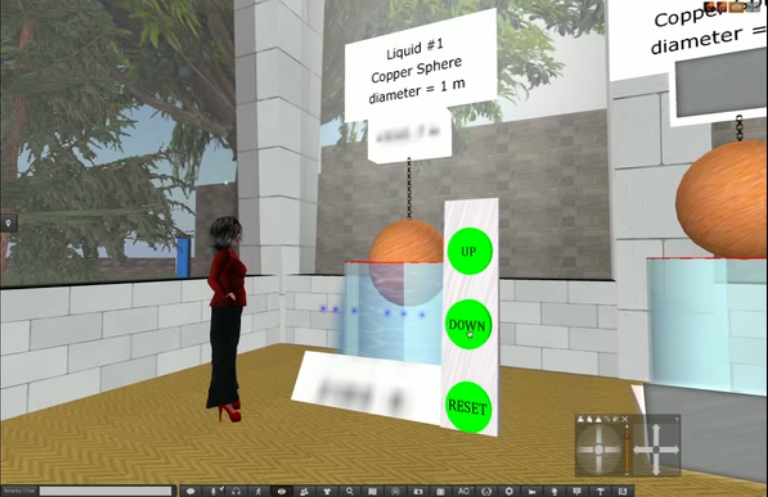
\includegraphics[width=1\linewidth]{fig 3.jpg}
    \caption{An avatar causes a copper sphere to incrementally submerge in a tank of some unknown liquid. The upper scale indicates the tension in the chain supporting the sphere, and the lower scale shows the increase in the downward force exerted by the liquid}
\end{figure}

The Webassign homework problem that goes with this activity is, in part:

\subsection*{Liquid 1}
Reset the sphere’s position. It should not be touching the liquid. Now click the “Down” button 10 times. This will submerge the sphere halfway.

\begin{enumerate}[label=\alph*)]
    \item What is the volume of the submerged part of the sphere? (Include units.)
    \item As the sphere sinks, liquid splashes out of the tank. This is the displaced liquid. What volume of liquid overflowed the tank? (Include units.)
    \item  How much buoyant force is the liquid applying to the sphere? (Include units.)
    \item  What is the relationship between the buoyant force on an object and the displaced liquid? Choose the correct phrase. The buoyant force is always equal to the volume of the displaced liquid. The buoyant force is always equal to the mass of the displaced liquid. The buoyant force is always equal to the weight of the displaced liquid.
    \item  What is the weight of the displaced liquid? (Include units.)
    \item  What is the mass of the displaced liquid? (Include units.)
    \item  Calculate the density of the liquid. (Include units.)
    \item  Calculate the specific gravity of the liquid.
    \item  What do you think this liquid probably is? (Type the name of the liquid in this box.)
\end{enumerate}

In the real life lab, this is a complicated set up. There is a scale suspended above the beaker of water, and the beaker rests on another scale. This lab displays a fair amount of Wieman and Perkins’s (2005) “peripheral information,” particularly since most lab scales yield measurements in grams, and force is measured in units called newtons, necessitating a calculation for every force.

To someone who is familiar with Archimedes’ Principle performing this lab seems straightforward. Students experience it as anything but simple, and what often happens is that one person performs the lab, reading off the measurements to the other members of his team, who are concerned principally with writing everything down correctly. There is pressure to finish in the allotted time, and careful observation and reflection is impossible.

The Second Life lab cleans up the equipment by removing extraneous support rods, strings, and puddles of water. Students are presented with a very large (1 meter diameter) copper sphere which they can incrementally lower into a tank of an unknown liquid. Questions in the assignment lead them through an inquiry process that involves taking data and answering questions about it as they go. They see that as the sphere is lowered into the liquid, each increment causes liquid to splash out of the tank. Each increment changes the force measurements in the scales, which are correctly calibrated in newtons.

Accelerated motion in 1 dimension. One of the fundamental characteristics of a moving object is its acceleration. Students commonly confuse the notion of acceleration with that of velocity. This activity, both in the lab and in Second Life, is used to reinforce the idea that acceleration depends on a change of velocity and the time required for that change to occur.

\begin{figure}[h]
    \centering
    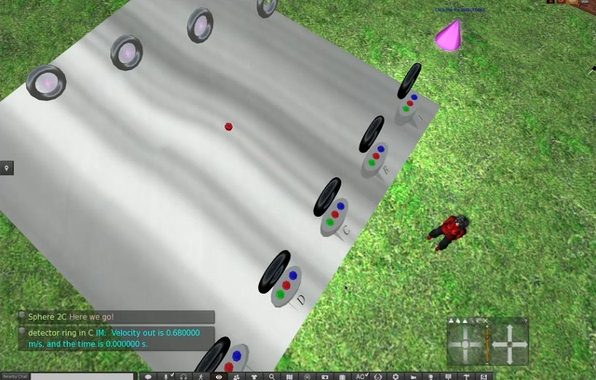
\includegraphics[width=1\linewidth]{fig 4.jpg}
    \caption{The bowling alley consists of 5 “alleys” of different lengths, with rings as detectors and timers of spheres which are pitched through them. Fifteen spheres have 15 accelerations.}
\end{figure}

This video shows an avatar creating spheres with are “thrown” through two rings in succession. The first ring measures the velocity of the sphere as it passes through the center and the sets the timer to 0. The second ring measures the velocity of sphere as it passes through the center, and reports on the time that was required for the sphere to transit between the rings. There are five stations, each with a different ring separation, and each with three spheres. Students answer questions like this one on Webassign.

Station A: Sphere 1 (Green button):
\begin{enumerate}[label=\alph*)]
    \item  What was the speed of the sphere when it went through the first ring? It will tell you in chat.
    \item  And what was the speed of the sphere when it went through the second ring?
    \item  Did the velocity change?
\begin{itemize}
    \item   Yes, it was slowing down.
    \item Yes, it was speeding up.
    \item  No, the velocity remained constant.
\end{itemize}
    \item So, was the sphere accelerating or not?
  \begin{itemize}
    \item It was accelerating.
    \item It was not accelerating.
  \end{itemize}
    \item  And how much time did it take to move between the rings?
    \item  If the sphere was accelerating, calculate the acceleration. If it was not accelerating, enter 0.
\end{enumerate}

Their purpose of this lab is to drive home the basic definition of acceleration. In the lab, students have measured the time for a cart to transit between two photogates and have calculated its acceleration; in fact this is a lab common to all elementary physics classrooms. Students do this activity, after first figuring out how the photogates work, and concentrate on gathering data and displaying

it appropriately in tables, and showing all of their calculations. It’s a good introduction, but many find it difficult to explain what acceleration is after this lab, although they can often calculate it. They do their calculations at a remove from the equipment. What did the cart look like as it rolled through the photogates. It was moving, but how?

The Second Life homework gives students practice in calculating with new data (far more practice than lab time allows). It removes the distraction of coping with setting up unfamiliar lab equipment, and it presents a picture of 15 accelerating objects that can be summoned and observed endless times. The questions require students to observe the moving spheres in order to answer, and to reflect directly on the spheres’ changes of velocity. This homework supports and reinforces what students have done in the lab. This “bowling alley” is also used for kinematics work, calculating the separation of the rings, and for studying dynamics, determining the force that would be necessary to accelerate the sphere.

Density. Density, mass, weight, and volume are related concepts that are frequently confused. Are large things more dense than small things? Are heavy things more dense than light things? Of course, the answer to both of those questions is “That depends!”

In this assignment, students create 4 pairs of objects and answers the following questions. This is only a partial assignment.

\begin{figure}[h]
    \centering
    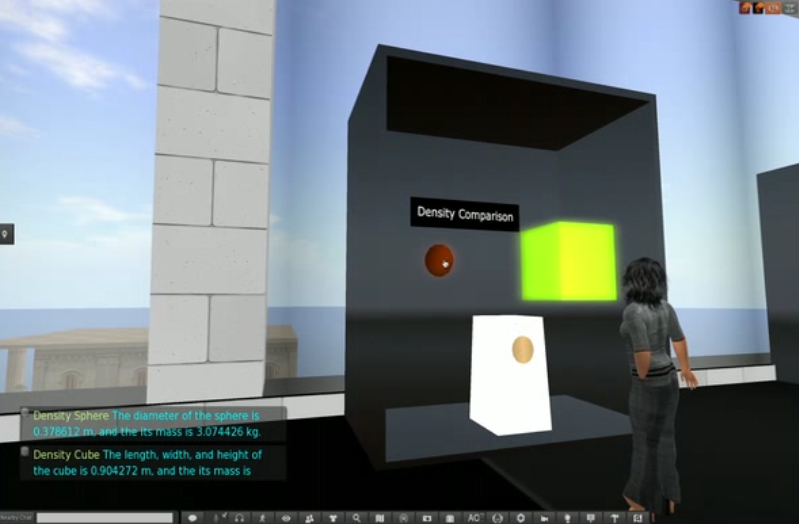
\includegraphics[width=1\linewidth]{fig 5.jpg}
    \caption{An avatar creates a sphere and a cube, which provide their dimensions and masses. This can be done any number of times. The cubes’ and spheres’ dimensions are randomly determined by the script which creates them.}
\end{figure}

\newpage
Question 1:

\begin{enumerate}[label=\alph*)]
    \item  Enter the diameter of the sphere:
    \item  Enter the mass of the sphere:
    \item  Calculate the volume of the sphere:
    \item  Calculate the density of the sphere:
    \item  Enter the length of the sides of the cube:
    \item  Enter the mass of the cube:
    \item  Calculate the volume of the cube: (If the volume is less than 1, use scientific notation with two decimal places,
    \item ie 0.0643 = 6.43e-2)
    \item Calculate the density of the cube: (If the density is less than 1, use scientific notation with two decimal places, ie 0.0643 = 6.43e-2)
    \newpage
    \item  Which object is heavier, the sphere or cube?
\begin{itemize}
    \item Sphere
    \item Cube
    \item They are equal.
\end{itemize}
    \item  Which object is larger, the sphere or the cube?
\begin{itemize}
    \item Sphere
    \item Cube
    \item They are equal.
\end{itemize}
    \item  Which one has more density, sphere or the cube?
\begin{itemize}
    \item Sphere
    \item Cube
    \item They are equal.
\end{itemize}
\end{enumerate}

Students are asked to make a general rule, if possible, relating greater density to greater or lesser volume or greater or lesser mass. Of course, there is no such rule. Most of the students realize this after examining their data.

\end{large}
\clearpage
\section*{REFERENCES}\par 

\leftskip 0.25in
\parindent -0.25in 
Coming of Age in Second Life: An Anthropologist Explores the Virtually Human (21 April 2008) by Tom Boellstorff

Edwards, C. (2006) Another world [3D virtual world]. Engineering \& Technology, Volume 1, Issue 9, 28-32. DOI: 10.1049/et:20060904

Domin, D. S., (1999). A Review of Laboratory Instruction Styles. Journal of Chemical Education. 76 (e.g. 2), pp.543-547 

dos Santos, R. (2009). Second Life Physics: Virtual, Real or Surreal?. Journal For Virtual Worlds Research, 2(1). doi:10.4101/jvwr.v2i1.383 

dos Santos, R. P. Second Life As A Platform For Physics Simulations And Microworlds: An Evaluation. Retrieved October 28, 2013 from \url{http://www.fisicainteressante.com/}

H Lang, M Stinson, F Kavanagh, Y Liu, and M Basile (1999) Learning styles of deaf college students and instructors’ teaching emphases. Journal of Deaf Studies and Deaf Education, 4 (1): 16-27 doi:10.1093/deafed/4.1.16 

Lord, Thomas, Orkwiszewski, Terri. (2006) Moving From Didactic to Inquiry-Based Instruction In A Science Laboratory. The American Biology Teacher, 68(6):342-345. 2006 DOI:10.1662/0002-7685(2006)68[342:DTIIIA]2.0.\\CO;2 

Marschark, Marc, Knoors, Harry (2012) Educating Deaf Children: Language, Cognition, and Learning. Deafness \& Education International, Vol. 14 No. 3, September, 2012, 136–160, DOI:10.1179/1557069X12Y.0000000010

McKeachie, W.J., Pintrich, P.R., Lin, Y.G., \& Smith, D.A. (1987). Teaching and learning in the college classroom: A review of the literature. Ann Arbor: National Center for Research to Improve Postsecondary Teaching and Learning, The University of Michigan. 

Merchant, Z., Goetz, E. T., Cifuentes, L., Keeny-Kennicutt, W., Davis, T. J., (2014). Effectiveness of virtual reality-based instruction on students’ learning outcomes in K-12 and higher education: A meta-analysis.. Computers \& Education. 70, pp.29-40

Prince, Michael. (2003)Does Active Learning Work? A Review of the Research. Journal of Engineering Education 93.3 (2004):223-31.ProQuest. Web. 24 Oct. 2013.


Wieman, Carl, Perkins, Katherine (2005) Transforming Physics Education. Physics Today, Vol 58, Issue 11, November 2005, 36-41, DOI: 10.1063/1.2155756 

\clearpage

\leftskip 0in
\parindent 0in 
\begin{large}
\section*{BIOGRAPHICAL STATEMENTS}
Vicki Robinson is an Associate Professor at the National Technical Institute for the Deaf at Rochester Institute of Technology. Since 1978, she’s taught various entry-level physics courses and investigated new instructional-delivery technologies as they relate specifically to deaf students’ learning in physics.

\end{large}
\end{document}
